\chapter{Introductie Python}
\begin{fquote}[John Cleese][Monty Python][1975]
	And now for something completely different.
\end{fquote}

We stappen nu een compleet nieuwe programmeer-wereld in, namelijk die van \textit{Python}. \textit{Python} is een programmeertaal van hogere orde ten opzichte van \textit{C}. Hoe hoger de orde van een programmeertaal, des te verder de taal weg staat van daadwerkelijke machine-instructies.

Python is een favoriete taal voor menig programmeur, omdat het redelijk makkelijk te leren is, de code compact en leesbaar is, voor een enorm scala aan projecten in te zetten is (van websites en kunstmatige intelligentie tot scripts en Raspberry Pi's), en de enorme gemeenschap die de taal gebruikt en ook verder uitbreidt d.m.v. softwarebibliotheken (hierover later meer). 

Zoals altijd komen al deze voordelen ook met enige nadelen (waar omheen gewerkt kan worden). \textit{Python} is bijv. een stuk langzamer dan \textit{C} (afhankelijk van de toepassing zo'n 2 tot 100 keer), vandaar dat we met dit vak afstappen van de inmiddels bekende \textit{Arduino} en overstappen naar de veel krachtigere \textit{Raspberry Pi} en je eigen laptop/PC.

\section{Installatie}\index{Installatie}
\vspace{5mm} 
\begin{exercise}
Installeer de laatste versie van Python op je eigen laptop via: \url{https://www.python.org/downloads/}

Let er bij het installeren op dat je alle vinkjes aanzet (vooral $pip$ is een belangrijke).
\end{exercise}

\section{Interpreter}\index{Interpreter}
Nu dat de installatie van \textit{Python} is voltooid is het tijd om te checken of alles goed is gegaan. Open een \textit{shell prompt} (onder Windows: startmenu -> zoeken naar \textit{cmd} of \textit{PowerShell}, onder Linux en Mac OS: open de \textit{Terminal}). Dit is een interactieve scherm waarmee je via tekst commando's kunt uitvoeren. De \textit{Python} interpreter is nu één van die commando's, typ \textit{python3} en druk dan op enter. Als het goed is zie je iets vergelijkbaars als in Figuur \ref{fig:interpreter} (Als deze niet werkt, probeer eens enkel \textit{python} te typen).

\begin{figure}[h!]
\centering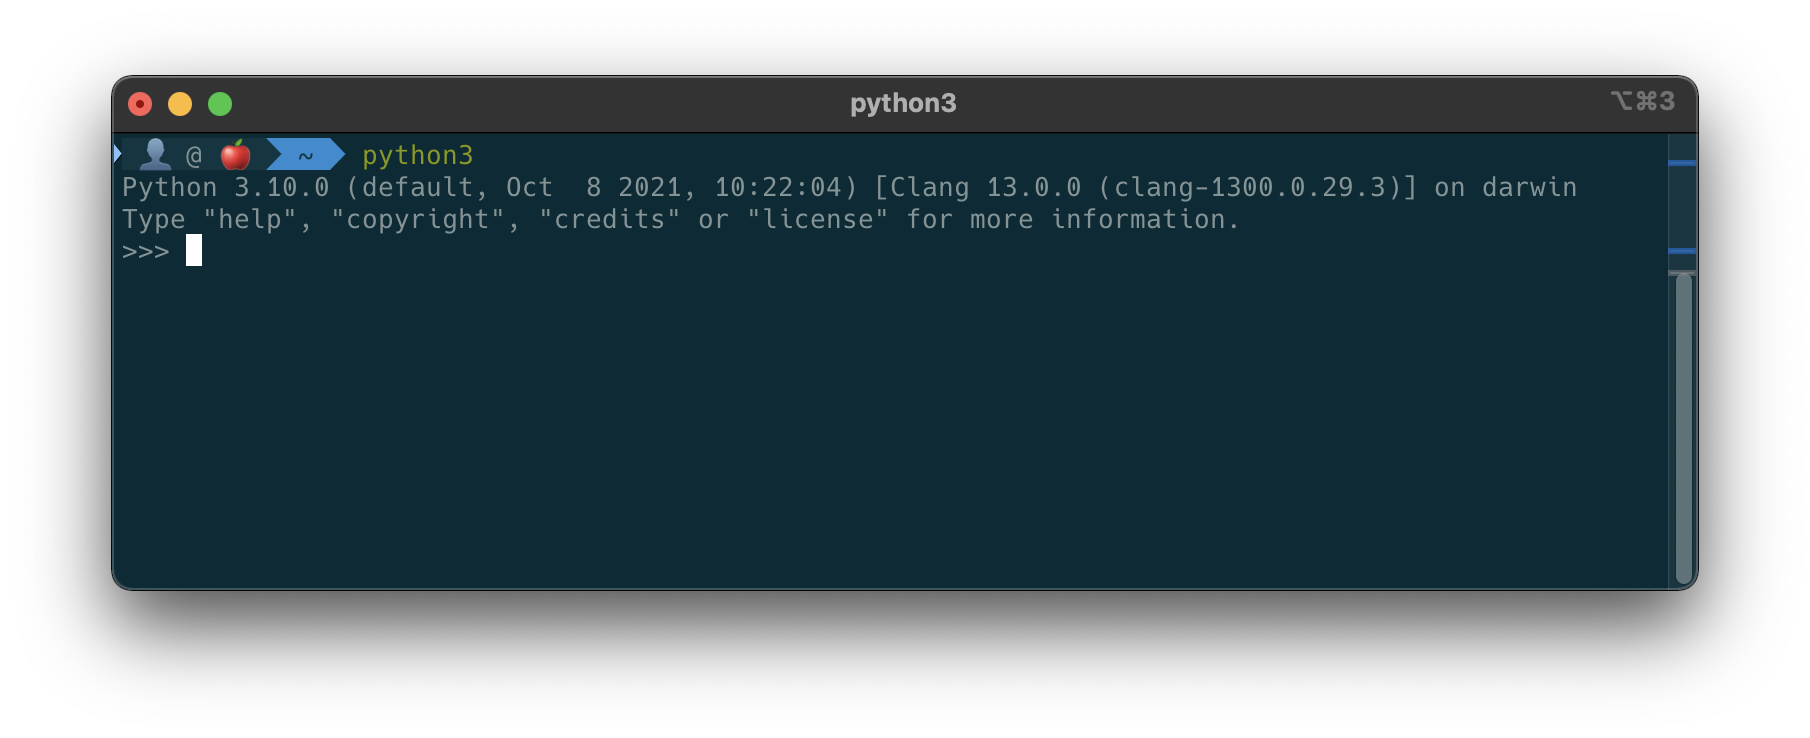
\includegraphics[scale=0.42]{Pictures/chapter04/python_shell.png}
\caption{De \textit{Python} interpreter, met versie $3.10.0$}
\label{fig:interpreter} % Unique label used for referencing the figure in-text
%\addcontentsline{toc}{figure}{Figure \ref{fig:webserver}} % Uncomment to add the figure to the table of contents
\end{figure}

\begin{exercise}
Check of de versie van \textit{Python} die je geïnstalleerd hebt overeen komt met de versie die de interpreter aangeeft.
\end{exercise}

De interpreter is een super handig stukje software, waarin je \textit{Python} code, regel voor regel in kunt typen, zodat je kunt checken of de code doet wat je verwacht. 
\begin{exercise}
Traditiegetrouw begint het leren van een nieuwe programmeertaal altijd met uitvoeren van \textit{Hello world!}. Typ in het scherm het volgende in, en zie wat er gebeurt:
\begin{python}[numbers=none]
print('Hello World!')
\end{python}
Hoeveel regels code zou je hier nodig voor zijn bij de Arduino?
\end{exercise}

\begin{remark}
Als er in dit document een stukje voorbeeld code, de regel begint met '$>>>$', dan wordt deze code ingetypt in de interpreter. De opvolgende regel zonder '$>>>$' is dan de uitvoer van de interpreter. Bijvoorbeeld:
\begin{python}
>>> print('Hello World!')
Hello World!
\end{python}
Elk ander stukje voorbeeld code zullen (gedeeltes van) scripts zijn. 
\end{remark}

\section{Editor}\index{Editor}
Elke regel op deze manier intypen is natuurlijk voor grotere programma's niet ideaal, deze slaan we dan ook op in \textit{Python} scripts (bestanden met als extensie $.py$). Deze kun je in principe gewoon maken in een tekst-editor, maar net als bij de \textit{Arduino} werkt het een stuk fijner in een ontwikkelomgeving. Voor \textit{Python} zijn er een flink scala aan zulke ontwikkelomgevingen (ook wel: IDE's). En je bent uiteraard helemaal vrij om zelf je favoriet daarin te kiezen om de opdrachten gedurende dit vak uit te werken.

Voor de beginners kan ik de IDE \textit{Thonny} aanraden: \url{https://thonny.org/}. \par 
Deze heeft naast een gebruikersvriendelijke interface, ook enkele handige tools aan boord die later van pas gaan komen. Bijkomend voordeel is dat dit programma ook standaard wordt meegeleverd met de \textit{Raspberry Pi}. Tijdens de les zullen de voorbeelden ook worden gegeven aan de hand van \textit{Thonny}.
\begin{exercise}
Installeer een \textit{Python} ontwikkelomgeving.
\end{exercise}

\section{Data Types}\index{Data Types}
Net als in \textit{Arduino C}, zijn in \textit{Python} verschillende datatypes beschikbaar, die de basis vormen van de taal. Zo zijn er gehele getallen (vergelijkbaar met \textit{int}s in \textit{C}):

\begin{python}
>>> x = 3
>>> y = 4
>>> x + y
7
\end{python}
Wat direct opvalt, is dat je in \textit{Python} dus niet hoeft aan te geven welk data type je wilt gebruiken. De taal 'snapt' dit automatisch. De puntkomma aan het eind, die bij \textit{C} elke regel code afsluit, wordt hier niet gebruikt. Verder kun je (op vergelijkbare manier als in \textit{C}) de getallen ook schrijven in binair en hexadecimaal:
\begin{python}
>>> x = 0b101
>>> x
3
>>> y = 0x1A
>>> y
26
\end{python}

Naast gehele getallen zijn er ook uiteraard komma-getallen (vergelijkbaar met \textit{float}s in \textit{C}):
\begin{python}
>>> x = 3.0
>>> y = 4.5
>>> x / y
0.6666666666666666
\end{python}

Ook kent de taal Booleans, die enkel \pyth{True} of \pyth{False} kunnen zijn. Waarmee digitale operaties kunnen worden uitgevoerd (vergelijkbaar met de \textit{bool}s uit \textit{C}):
\begin{python}
>>> a = True
>>> b = False
>>> a and not b
True
\end{python}

\newpage

en voor nu als laatste: \pyth{str}, de \textit{string} waarmee tekst kan worden toegekend aan een variabele. (Vergelijkbaar met de \textit{String}s uit \textit{C}):
\begin{python}
>>> a = 'Hello'
>>> b = "World!"
>>> a + ' ' + b  # Plak beide aan elkaar, met een spatie ertussen.
'Hello World!'
\end{python}
Het maakt bij \pyth{str}s dus ook niet uit of je nu enkele (\pyth{'}) of dubbele (\pyth{"}) aanhalingstekens gebruikt. Verder zie je hier ook voor het eerst een regel commentaar, die je kunt toevoegen na een hekje (\pyth{#}).

\begin{exercise}
\textit{Python} heeft een aantal operatoren voor getallen die bekend voor zullen komen: \pyth{+}, \pyth{-}, \pyth{*} om resp. getallen op tellen, af te trekken en te vermenigvuldigen. Maar kent ook een aantal die wat minder voor de hand liggen. Probeer er achter te komen wat \pyth{%} en \pyth{**} doen.
\end{exercise}

Naast dat het bij \textit{Python} dus niet nodig is om van te voren te specificeren welk datatype je gaat gebruiken voor een variabele, kun je ook variabelen van type laten veranderen gedurende het programma. Dit is voor de leesbaarheid niet aan te bevelen, maar het laat wel zien dat \textit{Python} veel losser om gaat met de verschillende types dan dat we gewend waren met \textit{C}:
\begin{python}
>>> x = 12  # x is nu een int
>>> x
12
>>> x = 'abc'  # En vanaf hier een str
>>> x
'abc'
\end{python}

\section{If/Else statements}\index{If/Else statements}
Een van de meest voorkomende en belangrijke dingen die er gebeurt in een programma, is keuzes maken op basis van condities. In z'n meest eenvoudige manier, doen we dat met een \pyth{if}-statement:
\begin{python}
a = 200
if a > 100:
	print('conditie is True!')
	print('a is groter dan 100')
\end{python}
De \pyth{if}-statement is opgebouwd uit $3$ delen: allereerst het woordje \pyth{if}. Dan gevolgd door een conditie (ook wel expressie genoemd), en uiteindelijk een dubbele punt \pyth{:}. Die conditie is het meest interessant, als daar namelijk \pyth{True} uitkomt worden de volgende regels code uitgevoerd, komt er \pyth{False}, gebeurt er in dit geval niets. 

\begin{remark}
\textbf{Let op:} Ook hier is de schrijfwijze van \textit{Python} weer een stuk compacter dan in \textit{C}: waar je bij die laatste vaak gekrulde haken $\{$, $\}$ ziet, gebruikt \textit{Python} juist inspringing om duidelijk te maken wat bijv. bij een statement hoort. Voor het inspringen gebruik je $4$ spaties of een tab. Dit is dus \textbf{essentieel} voor de werking van je programma! Zie bijv. het volgende voorbeeld:
\begin{python}
a = 200
if a > 100:
	print('conditie is True!')
print('a is groter dan 100')
\end{python}
Hier wordt dus regel $3$ enkel uitgevoerd als \pyth{a>100} is, maar regel $4$ altijd. Let dus goed op bij het inspringen van code!
\end{remark}

De \pyth{if}-statement kan uitgebreid worden met een \pyth{else}-clausule, die uitgevoerd wordt als de conditie \pyth{False} is.
\begin{python}
a = 200
if a > 100:
	print('conditie is True!')
	print('a is groter dan 100')
else:
	print('conditie is False!')
	print('a is kleiner of gelijk dan 100')
\end{python}

\textbf{Tip:} Als je niet zeker van jezelf bent wat er precies uit de conditie komt van je \pyth{if}-statement, kun je hier dus handig gebruik maken van de interpreter:
\begin{python}
>>> a = 200
>>> a > 100
True
\end{python}

Soms wil je meerdere condities checken, dit kan met \pyth{elif} (dit staat voor een samentrekking van \pyth{else if}). Je kan daarvan zoveel als je wil in je \pyth{if}-statement stoppen:
\begin{python}
a = 200
if a > 100:
	print('a is groter dan 100')
elif a == 100:
	print('a is precies 100!')
else:
	print('a is kleiner dan 100')
\end{python}
\begin{exercise}
Typ het bovenstaande over in je editor, sla het op als een \textit{.py} bestand. Probeer het programma te starten (In \textit{Thonny}: Zoek naar de groene play knop, genaamd 'run'). Waar kun je de uitvoer van het programma zien?
\end{exercise}

\section{Input/Output}\index{Input/Output}
Zo'n programma als hierboven, die afhankelijk van de waarde van een vast getal iets uitvoert is natuurlijk niet superspannend. Het wordt al interessanter als je input van de gebruiker van het programma kunt vragen. Dat doe je met de functie \pyth{input()}:
\begin{python}
print('Typ iets: ')
a = input()
print('Je typte: ' + a)
\end{python}

\begin{remark}
\textbf{Tip:} Regel $1$ en $2$ zijn ook te combineren tot \pyth{a = input('Typ iets: ')}.
\end{remark}

\begin{exercise}
Voer het bovenstaande stuk code uit. Merk op dat halverwege het programma wordt gepauzeerd. Wat moet je doen om het programma weer verder te laten gaan?
\end{exercise}

\begin{remark}
\textbf{Tip:} In plaats van regel $3$, kun je ook gebruik maken van de zogeheten \textit{f-strings}. Dit is een wat efficiëntere manier van schrijven, maar doet precies hetzelfde: 
\begin{python}
print(f'Je typte: {a}')
\end{python}
Vooral bij langere wat langere strings, kan dit de leesbaarheid van je code bevorderen.
\end{remark}

\newpage 

\section{Huiswerkopdrachten}\index{Huiswerkopdrachten}
\vspace{2mm} 
\begin{exercise} \label{exc4:exc1}
Maak een programma dat de gebruiker om zijn naam vraagt. Groet hierna de gebruiker in de vorm van \textit{"Hallo, <naam>!"}.
\end{exercise}

\begin{exercise}
Breid het programma van opdracht \ref{exc4:exc1} uit, zodat het programma je schreeuwend begroet: \textit{"HALLO, <NAAM>!"}. 

\textbf{Tip:} Zoek zelf uit hoe je een string naar hoofdletters kunt om te zetten, kijk gerust op \href{https://www.w3schools.com/python/python_ref_string.asp}{deze link} om te zien welke functies je op een string kunt uitvoeren.
\end{exercise}

\begin{exercise}
Schrijf een programma dat de gebruiker vraagt om de straal ($r$) van een cirkel in te typen. Geef daarna de omtrek (= $2*r*\pi$) en de oppervlakte (= $r^2*\pi$) op basis van de straal. 

\textbf{Tip 1:} Alles wat de gebruiker intypt, en je afvangt met \pyth{input()} is van het type string. Om van een string met cijfers, een daadwerkelijk getal te maken, gebruik je de functie \pyth{int()}. Bijv. \pyth{x = int('123')}.

\textbf{Tip 2:} Zet bovenin je programma \pyth{import math}, je hebt daarna toegang tot allerlei wiskundige functies. Zo ook \pyth{math.pi} en \pyth{math.pow()}.
\end{exercise}

\begin{remark}
\textbf{Tip:} Als je niet zeker van jezelf bent wat voor type een variabele krijgt, kun je ook hier handig gebruik maken van de interpreter en de functie \pyth{type()}:
\begin{python}
>>> a = 'een string'
>>> b = 4
>>> type(a)
<class 'str'>
>>> type(b)
<class 'int'>
\end{python}
\end{remark}

\begin{exercise}
Breid het programma van opdracht \ref{exc4:exc1} uit, zodat het programma de gebruiker vraagt om achtereenvolgens z'n voornaam, achternaam, geslacht en leeftijd. 

Groet hierna de gebruiker in de vorm \textit{"Hallo, <voornaam>!"}. 

Is de persoon in kwestie echter ouder dan $50$, gebruik dan een formelere begroeting op basis van zijn of haar geslacht: \textit{"Gegroet, Mr. <achternaam>!"} of \textit{"Gegroet, Mevr. <achternaam>!"}
\end{exercise}

\begin{exercise}
Maak een programma dat de gebruiker vraagt om een getal, geef daarna aan of dat getal even of oneven is.
\end{exercise}

\begin{exercise}
Schrijf een programma dat de gebruiker vraagt om 2 getallen in te voeren, print daarna de grootste van de twee op het scherm. 
\end{exercise}

\begin{exercise}
Schrijf een programma dat de gebruiker vraagt om een getal. Dit getal correspondeert met een dag in de week ($1$ = maandag, $2$ = dinsdag, etc.). print de correspondeerde dag op het scherm. Als de gebruiker een getal groter dan $7$ of kleiner dan $1$ invoert, geef dan een 'error'.
\end{exercise}

